\begin{frame}[plain]
    \begin{center}
        \vspace{48pt}
        {\huge\bf 距離センサーを使ってみよう}
    \end{center}
\end{frame}

\begin{frame}[fragile]
    \frametitle{距離センサーを\\ピンにつけてみよう}
    \begin{columns}
        \begin{column}{0.48\textwidth}
            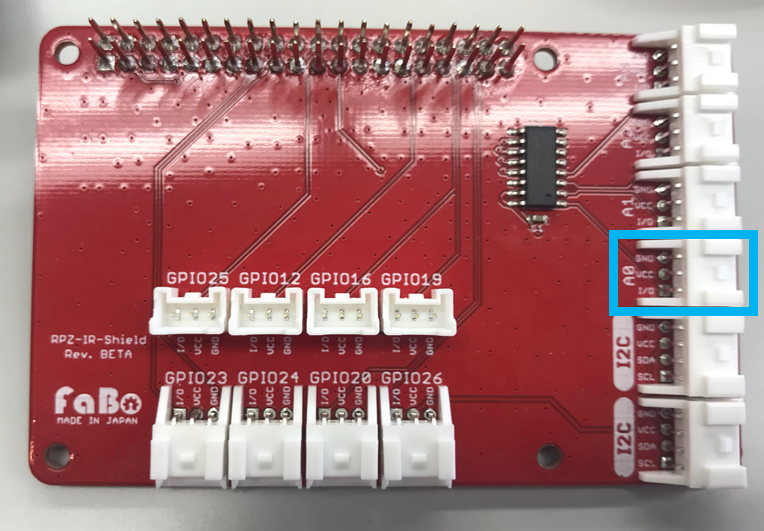
\includegraphics[width=\textwidth]{images/chap05/text05-img030.png} 
        \end{column}
        \begin{column}{0.48\textwidth}
            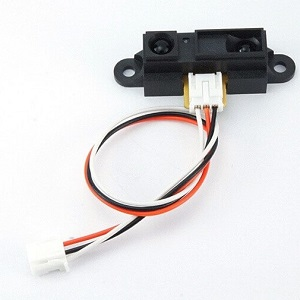
\includegraphics[width=\textwidth]{images/chap05/text05-img023.jpg} 
        \end{column}
    \end{columns}
    \begin{itemize}
        \item A0と距離センサーをつなげてみよう
        \item HSPで\textasciitilde/05/kyori.hspを動かしてみよう
    \end{itemize}
    \textpageref{18}
\end{frame}

\begin{frame}[fragile]
    \frametitle{距離センサーのプログラム}
    \begin{lstlisting}[title=\textasciitilde/05/kyori.hsp]
    #include "hsp3dish.as"
    #include "rpz-gpio.as"

    spiopen 0

    *main

	    data = spiget(0,0)
	    kyori = -1*(data*5000/1023)/36+845/9
	    res = "距離 : "+kyori
	
	    redraw 0
	    font "",20
	    pos 30,30
	    mes res
	    redraw 1

	    wait 10
	    goto *main

    spiclose 0
    \end{lstlisting}
    \textpageref{18}
\end{frame}

\begin{frame}
    \frametitle{距離を求める式の修正}
    修正前 kyori = -1*(data*5000/1023)/36+845/9\\
    \vspace{20pt}
	修正後 kyori = 3952640 / (875*data + 22272)
\end{frame}

\begin{frame}[plain]
    \begin{center}
        \vspace{48pt}
        {\huge\bf 有機ELディスプレイを使ってみよう}
    \end{center}
\end{frame}

\begin{frame}
    \frametitle{有機ELディスプレイ}
    \begin{center}
        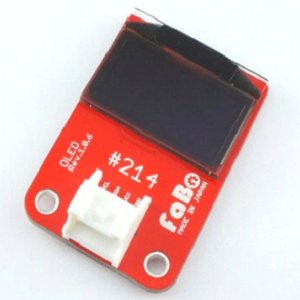
\includegraphics[width=0.4\textwidth]{images/chap05/text05-img025.png}
        \begin{itemize}
            \item 文字(記号や英数字)を画面に表示する
            \item ここでは日本語を表示できない
        \end{itemize}
    \end{center}
    \textpageref{20}
\end{frame}

\begin{frame}[fragile]
    \frametitle{有機ELディスプレイを\\ピンにつけてみよう}
    \begin{columns}
        \begin{column}{0.48\textwidth}
            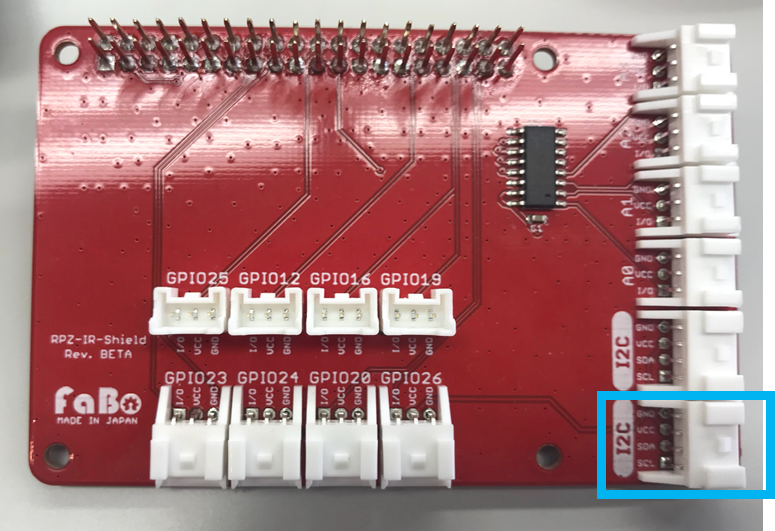
\includegraphics[width=\textwidth]{images/chap05/text05-img033.png} 
        \end{column}
        \begin{column}{0.48\textwidth}
            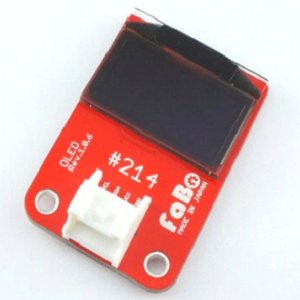
\includegraphics[width=\textwidth]{images/chap05/text05-img025.png} 
        \end{column}
    \end{columns}
    \begin{itemize}
        \item 有機ELディスプレイとI2Cをつなげてみよう
        \item HSPで\textasciitilde/05/oled.hspを動かしてみよう
    \end{itemize}
    \textpageref{20}
\end{frame}

\begin{frame}[fragile]
    \frametitle{有機ELディスプレイを使った\\プログラム}
    \begin{lstlisting}[title=\textasciitilde/05/oled.hsp]
    #include "hsp3dish.as"
    #include "rpz-gpio.as"

    redraw 0
    font "",20
    pos 20,20
    mes "有機ELディスプレイを見てね\nカンマ(,)で改行するよ"
    redraw 1

    oled "Good Morning,Good Bye,Good Afternoon"

    wait 100
    \end{lstlisting}
    \textpageref{20}
\end{frame}

\begin{frame}[fragile]
    \begin{exampleblock}{問題を解いてみよう}
    \begin{itemize}
        \item 教科書19ページ 問題5-8(1問)
        \item 教科書21ページ 問題5-9(2問)
    \end{itemize}
    \end{exampleblock}
\end{frame}